

\chapter{Resultados} \label{chap:resultados}

\begin{figure}[H]  % <-- Este cambio es clave para que no se brinque
	\centering
	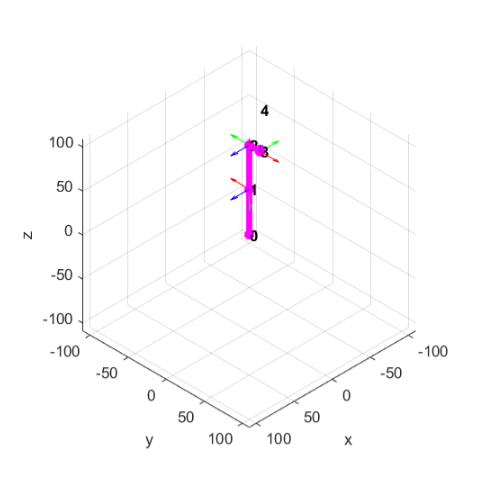
\includegraphics[width=0.7\linewidth]{img/grafica1directa}
	\caption{}
	\label{fig:grafica1directa}
\end{figure}

\begin{figure}[H]
	\centering
	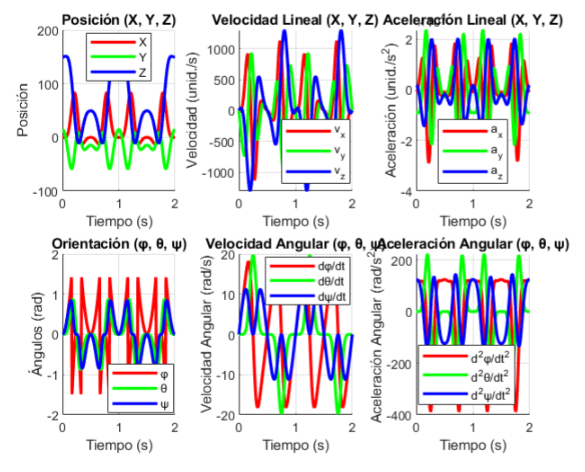
\includegraphics[width=0.7\linewidth]{img/imagen2directa}
	\caption{}
	\label{fig:imagen2directa}
\end{figure}

\begin{figure}[H]
	\centering
	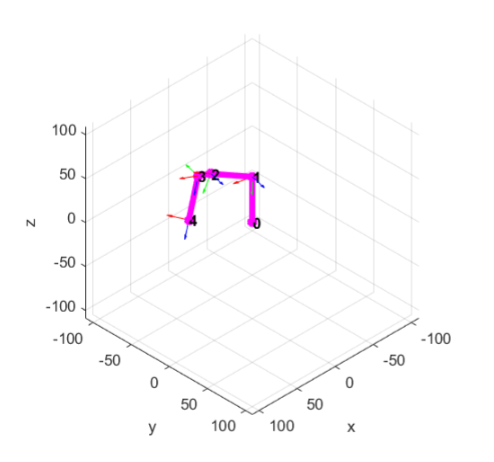
\includegraphics[width=0.7\linewidth]{img/inversa1}
	\caption{}
	\label{fig:inversa1}
\end{figure}

\begin{figure} [H]
	\centering
	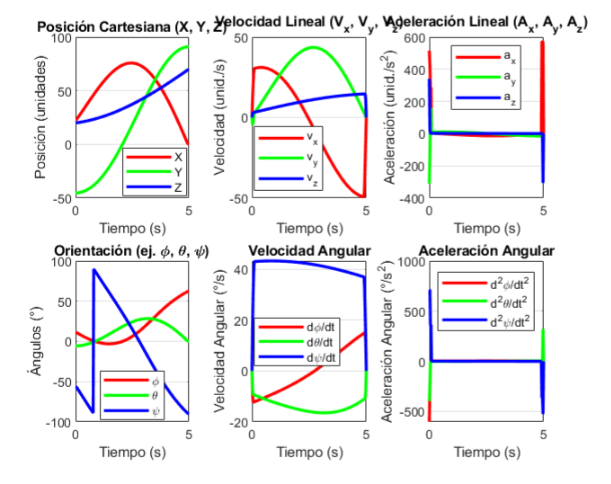
\includegraphics[width=0.7\linewidth]{img/inversa2}
	\caption{}
	\label{fig:inversa2}
\end{figure}

\begin{figure} [H]
	\centering
	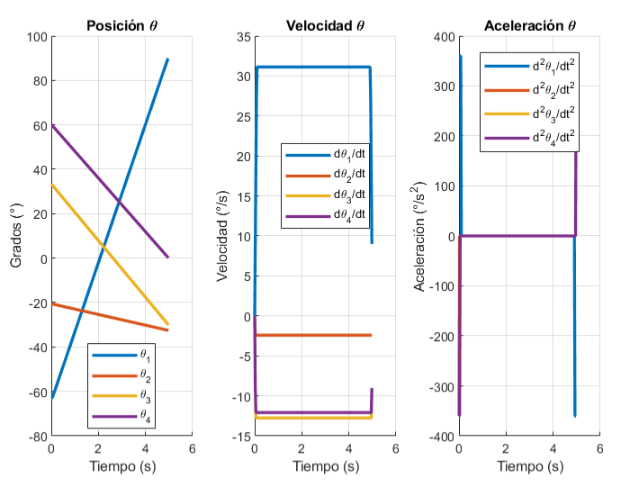
\includegraphics[width=0.7\linewidth]{img/inversa3}
	\caption{}
	\label{fig:inversa3}
\end{figure}

















